\section{Alts}
\label{sec:alt}

\inlineScala

We now consider alts.  We start by describing the high-level interactions
between an alt and channels, and how those interactions are implemented within
alts and channels.  We then outline how these interactions are modelled in
CSP, and describe a direct analysis of an alt and associated channels.

%%%%%%%%%%%%%%%%%%%%%%%%%%%%%%%%%%%%%%%%%%%%%%%%%%%%%%%

\subsection{High-level design}

An alt and its channels interact by calling operations on each other.  We call
the way they interact the \emph{alt protocol}.

We call the thread that is executing the alt the \emph{alt-thread}, and a
thread performing a send, receive or close operation in a channel a
\emph{channel-thread}.  The alt-thread calls (package-private) operations upon
relevant channels; and likewise, a channel-thread may call (package-private)
operations upon relevant alts.
When the alt-thread calls an operation on a channel, it uses the channel's
lock, so as to provide mutual exclusion; similarly, when a channel-thread
calls operations on the alt, it uses the alt's lock.

When an alt-thread executes an alt, it starts by locking the alt.  It then
registers, in turn, with each of the relevant ports whose guard evaluates to
|true|.  This registration tells the port that the alt is willing to
communicate, and asks the port whether it is also ready to communicate.  More
precisely, the alt-thread calls an operation
%
\begin{scala}
def registerIn(alt: AltT, index: Int): RegisterInResult[A]  
\end{scala}
%
on each of its in-ports, where |alt| is a reference to the calling alt, and
|index| is the index of the branch within the alt.\footnote{In the
  implementation, there is an additional parameter {\scalashape iter} that
  represents an iteration number when an alt is executed repeatedly; other
  operations described in this section have a similar parameter.  It is used
  only in assertions, checking that both components have the same value, and
  so we omit it from our analysis.}
%% , and |iter| is an iteration number
%% within a |serve| construct (used only for assertions).  
The operation returns a
result of type |RegisterInResult[A]|, where |A| is the type of data passed by
the port, of one of the following forms:
%
\begin{description}
\item[\rm{\scalastyle RegisterInSuccess(x)}:] the port is willing to
  communicate, and the alt has received~|x| from it;

\item[\rm{\scalastyle RegisterInWaiting}:] the port is not currently willing
  to communicate (the port stores the details of the registration in this
  case);

\item[\rm{\scalastyle RegisterInClosed}:] the port has been closed.
\end{description}
%
Similarly, the alt-thread calls an operation
%
\begin{scala}
def registerOut(alt: AltT, index: Int, value: () => A): RegisterOutResult
\end{scala}
on each of its out-ports, where |alt| and |index| are as for |registerIn|, and
|value| is a computation that, when evaluated, produces the value to be sent.
The operation returns a result of one of the following forms:
%
\begin{description}
\item[\rm{\scalastyle RegisterOutSuccess}:] the port is willing to
  communicate, and the alt has sent it a value;

\item[\rm{\scalastyle RegisterOutWaiting}:] the port is not currently willing to
  communicate (the port stores the details of the registration); 

\item[\rm{\scalastyle RegisterOutClosed}:] the port has been closed.
\end{description}

If one of the registrations is successful, the alt-thread releases the lock on
the alt (we explain the reason for this below).  It then deregisters from the
waiting branches, via operations |deregisterIn| and |deregisterOut|; this
tells the port that the alt is no longer willing to communicate (and the
channel removes the details of the registration).  The alt-thread then
executes the continuation of the successful branch.

\def\IP{\emph{IP}}
\def\OP{\emph{OP}}

Figure~\ref{fig:alt-1} gives an example: an alt first registers unsuccessfully
with an in-port~\IP; then it registers successfully with an out-port~\OP; and
finally it deregisters from~\IP.

%%%%%

\begin{figure}
\begin{center}
%\unScalaMid
\def\height{7.5} % height of sequence diagram
\def\gap{3.5} % gap between columns
\begin{tikzpicture}[yscale = 0.75, >= angle 60]
\draw (0,0) node[draw](alt){Alt};
\draw (alt) -- ++ (0,-\height);
\draw (alt)++(\gap,0) node[draw](c1){\IP};
\draw (c1) -- ++(0,-\height);
\draw (c1)++(\gap,0) node[draw](c2){\OP};
\draw (c2) -- ++(0,-\height);
% Lock
\draw (alt)++(0,-1) coordinate (lock); \drawloop(lock){\small lock}
% Register with IP
\draw[->] (lock)++(0,-1) -- node[above]{\scalashape\small registerIn}
  ++ (\gap,0);
\draw[<-] (lock)++(0,-2) -- node[above]{\scalashape\small RegisterInWaiting} 
  ++ (\gap,0);
% Register with OP
\draw[->] (lock)++(0,-3) -- node[above, near end]{\scalashape\small registerOut}
  ++ (2*\gap,0);
\draw[<-] (lock)++(0,-4) -- 
  node[above, near end]{\scalashape\small RegisterOutSuccess}
  ++ (2*\gap,0);
% Unlock
\draw (lock)++(0,-5) coordinate (unlock); \drawloop(unlock){\small unlock}
% Deregister with IP
\draw[->] (lock)++(0,-6) -- node[above]{\scalashape\small deregisterIn}
  ++ (\gap,0);
\end{tikzpicture}
\end{center}
\caption{Sequence diagram illustrating an alt that registers successfully with
  a port. \label{fig:alt-1}}
\end{figure}

%%%%%

If no registration is successful, and the alt-thread finds that every port is
closed or has a guard that is false, then it throws an |AltAbort| exception.
Otherwise, it waits (releasing the lock on the alt) for a callback from one of
the ports with which it is registered, of one of the following forms.
%
\begin{itemize}
\item If the alt is registered at the in-port of a channel, and another thread
  tries to send on the channel, it calls
\begin{scala}
def maybeReceive(value: A, index: Int): Boolean
\end{scala}
%
on the alt, where |value| is the value it is trying to send to the alt, and
|index| matches the value provided during registration.  This asks
the alt whether it is still willing to receive from the in-port, and if so
completes the communication, storing |value| in the alt. 

\item If the alt is registered at the out-port of a channel, and another thread
  tries to receive on the channel, it calls
%
\begin{scala}
def maybeSend[A](index: Int): Option[A]
\end{scala}
%
This asks the alt whether it is still willing to send a value to the in-port,
and if so completes the communication.

\item If another thread closes the channel, it calls 
%
\begin{scala}
def portClosed(index: Int)
\end{scala}
\end{itemize}
%
Each of the callbacks uses the alt's lock, to ensure mutual exclusion. 
Callbacks are blocked during the registration phase, because the alt-thread
holds the alt's lock.  

If the alt receives a call of |maybeReceive| or |maybeSend|, it responds
positively to the first such call, returning |true| to a |maybeReceive|, or
|Some(x)| to a |maybeSend|, where~|x| is the value it sends.
The  callback operation wakes up the alt-thread, which then
deregisters from the remaining branches.
%
Finally, the alt-thread
executes the continuation of the successful branch.
%
Figure~\ref{fig:alt-2} gives an example of a successful callback of
|maybeSend| from an out-port with which the alt is registered.

\begin{figure}
\begin{center}
%\unScalaMid
\def\height{9.5} % height of sequence diagram
\def\gap{3.5} % gap between columns
\begin{tikzpicture}[yscale = 0.75, >= angle 60]
\draw (0,0) node[draw](alt){Alt};
\draw (alt) -- ++ (0,-\height);
\draw (alt)++(\gap,0) node[draw](c1){\IP};
\draw (c1) -- ++(0,-\height);
\draw (c1)++(\gap,0) node[draw](c2){\OP};
\draw (c2) -- ++(0,-\height);
% Lock
\draw (alt)++(0,-1) coordinate (lock); \drawloop(lock){\small lock}
% Register with IP
\draw[->] (lock)++(0,-1) -- node[above]{\scalashape\small registerIn}
  ++ (\gap,0);
\draw[<-] (lock)++(0,-2) -- node[above]{\scalashape\small RegisterInWaiting} 
  ++ (\gap,0);
% Register with OP
\draw[->] (lock)++(0,-3) -- node[above, near end]{\scalashape\small registerOut}
  ++ (2*\gap,0);
\draw[<-] (lock)++(0,-4) -- 
  node[above, near end]{\scalashape\small RegisterOutWaiting}
  ++ (2*\gap,0);
% Unlock
\draw (lock)++(0,-5) coordinate (unlock); \drawloop(unlock){\small unlock}
% Call back
\draw[<-] (lock)++(0,-6) -- node[above, near end]{\scalashape\small maybeSend}
  ++ (2*\gap,0);
\draw[->] (lock)++(0,-7) -- node[above, near end]{\scalashape\small Some(x)}
  ++ (2*\gap,0);
% Deregister with IP
\draw[->] (lock)++(0,-8) -- node[above]{\scalashape\small deregisterIn}
  ++ (\gap,0);
\end{tikzpicture}
\end{center}
\caption{Sequence diagram illustrating a successful callback from a
  port.  \label{fig:alt-2}}
\end{figure}

%%%%%

If the alt receives multiple callbacks to
|maybeReceive| or |maybeSend| (including during deregistration), it responds
negatively to all except the first, returning |false| or |None|, respectively.
%
If all the channels with which the alt is registered call |portClosed|, the
alt-thread is woken up, and it throws an |AltAbort|. 

%%%%%%%%%%%%%%%%%%%%%%%%%%%%%%%%%%%%%%%%%%%%%%%%%%%%%%%%%%%%

\subsection{Implementation details}

We now describe some details of the implementation. 
%%  Below we will use the
%% term ``alt-thread'' for the thread that is running the alt, and
%% ``channel-thread'' for a thread performing an operation in a channel that
%% makes a callback to the alt. 

%% Each call of an operation on a channel (registering or deregistering) uses that
%% channel's lock, to avoid races.  

The implementation of the alt is based on a monitor, more specifically a
monitor provided by the Java Virtual Machine (JVM).  (JVM monitors are more
efficient than SCL monitors, because they are implemented directly in the JVM;
however, they do not allow targeting of signals.)  

The alt-thread holds the alt's lock throughout the registration phase.  As
noted above, each callback operation has to obtain this lock, so those
operations are blocked until registration is complete.

However, it would be a mistake for the alt-thread to continue to hold the
alt's lock during deregistration, for this could lead to deadlocks.  Suppose
it did continue to hold the lock, and consider the case that the alt-thread is
trying to deregister from channel~$c$, at the same time that a channel-thread
is trying to perform a callback from~$c$: the channel-thread holds the lock
on~$c$, so the deregistration would be blocked; but the alt-thread would hold
the lock on the alt, so the callback would be blocked.  The alt-thread
therefore releases the lock during deregistration.

The implementation uses a variable |done| that is set to |true| when a
branch is found that is willing to communicate, either during registration or
as the result of a callback.  If a callback of |maybeSend| or |maybeReceive|
finds that |done| is |true|, it can return a negative result.  Otherwise, it
stores relevant information (like the value it is sending in the case of
|maybeReceive|, and the index of the relevant branch), evaluates the value to
be received in the case of |maybeSend|, sets |done| to |true|, signals to the
waiting alt-thread, and returns a positive result.

If the alt-thread fails to communicate during registration, and not all
ports are closed, it waits to receive a signal.  Then, if |done| is true, it
deregisters from other branches and runs the continuation of the relevant
branch.  Otherwise, if all ports are closed, it throws an |AltAbort|. 

%% Why not hold lock during registration??

We now describe how the implementation of channels is extended to deal with
alts.

Each channel has variables to store information about alts currently
registered there.  These are set by the |registerIn| and |registerOut|
operations. 

Recall from the Introduction that the ports of a channel may not be
simultaneously feasible in two alts.
The |registerIn| operation checks whether another alt is currently registered
with the channel (which would be an error), and if so throws an exception.  If
the channel is closed, it returns |RegisterInClosed|.  If there is a waiting
sender (corresponding to the variable |status| holding |Filled|), it acts like
a standard receive, setting status to |Read| and signalling to the sender, and
then returns a |RegisterInSuccess| result.  Otherwise it records the
registration, and returns |RegisterInWaiting|.

The |registerOut| operation is somewhat similar.  If there are waiting
receivers, it first waits for any current exchange to finish (i.e.~for
|status| to hold |Empty|).  If there are still waiting receivers, it continues
as for a standard send: it stores its value, sets |status| to |Filled| and
signals to a receiver.  It then waits on the |continue| condition for a
receiver to take the value, and then resets |status| to |Empty|.  This latter
wait is necessary to ensure correct synchronisation: without it, the value
could be taken by a new receiver that calls |receive| only after the
alt-thread has returned.

The deregister operations simply clear the information stored during the
earlier registration.

If a call of |send| or |sendWithin| finds that there is an alt registered at
the in-port, it calls |maybeReceive| on that alt, and reacts accordingly.
Calls to |receive| or |receiveWithin| act similarly, calling |maybeSend|.  

Finally, when a channel is closed, it calls |portClosed| on any registered alt. 

%%%%%%%%%%%%%%%%%%%%%%%%%%%%%%%%%%%%%%%%%%%%%%%%%%%%%%%%%%%%

\subsection{CSP modelling for alts}

\inlineCSP

We now describe how to model an alt and its interactions with channels, using
CSP\@.  Much of the construction of the model follows a similar form to the
model of a channel.  We highlight the main differences. 

A JVM monitor is modelled by a CSP module, in a similar way to an SCL monitor.
A process records which thread, if any, currently holds the lock, and which
threads are currently waiting for a signal.  One difference, however, concerns
a bug in the implementation of JVM monitors\footnote{%
  \url{https://docs.oracle.com/javase/8/docs/api/java/lang/Object.html#wait-long-}.}:
a thread that is waiting for a signal may resume, even though it has received
no signal!  This is known as a \emph{spurious wakeup}.  The alt implementation
guards against spurious wakeups by performing a suitable check when resuming
after a wait, and waiting again if appropriate.
%
Our CSP model of a monitor reflects the possibility of spurious wakeups: it
allows a waiting thread~|t| to resume either as the result of a signal, or a
spurious wakeup, modelled by the event |spuriousWakeup.t|.  We run this
monitor process in parallel with a \emph{regulator process}
\begin{cspm}
Reg = spuriousWakeup?t -> Reg |~| STOP
\end{cspm}
(equivalently, \CSPM{Reg = CHAOS(\{\|spuriousWakeup\|\})}).  
The effect of this combination is that 
spurious wakeups (nondeterminstically) might or might not happen.
%
This last point is important: spurious wakeups can happen, but they can't be
relied on to happen.  If we allowed unrestricted spurious wakeups in the
model, there is a danger that our analysis would seem to show that suitable
progress properties are satisfied, when in fact it is only spurious wakeups
that allow progress, and without them the system would get stuck.

We choose not to model the guards of alt branches, for we believe that doing
so would add a lot of complexity to the model, and cause FDR checks to take
longer, without adding much assurance.  The part of the implementation
concerning guards is rather straightforward: a branch whose guard is false is
simply ignored.  We think it is best to concentrate on the more difficult
parts of the implementation.

We also do not model the expression that generates the value to be sent in an
out-port branch, but just pick the value nondeterministically.  Likewise, we
do not model the continuations of branches, which are executed after the
communication itself.  Each continuation could contain arbitrary code (of the
correct type); but they are outside the operation of the alt itself.  Instead,
the model just records the index of the branch selected.
 
%% Finally, we do not model the |iter| parameter in the registration and
%% deregistration operations, since it is used only in assertions as sanity
%% checks, and would greatly increase the state space of the models.

%%%%%

\begin{figure}
\begin{center}
\def\height{10mm} % height of boxes
\def\chanW{15mm} % width of Channel boxes
\def\gap{0.1} % gap for stacked figure
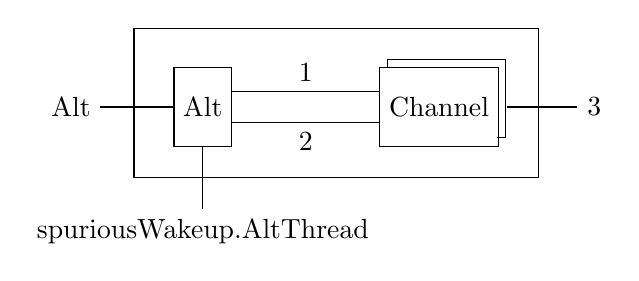
\begin{tikzpicture}
% Alt box
\draw(0,0) node[draw, minimum height = \height](alt){\cspmstyle Alt};
% Channel stacked box
\draw (3,0) node[draw, minimum height = \height, minimum width = \chanW](chan){
  \cspmstyle Channel};
\draw (chan.north west) ++ (\gap, 0.0) |- ++ (\chanW, \gap) |- 
  ++ (-\gap, -\height);
% Alt external interface
\draw (alt) -- node[left, at end]{\beginEnd{Alt}}  ++ (-1.3,0);
\draw (alt) -- node[below, at end]{\cspmstyle spuriousWakeup.AltThread} ++ (0,-1.3);
% Internal syncs
\path (alt.east) -- ++(0,-0.2) coordinate (a) -- ++(0,0.4) coordinate (aa);
\path (chan.west) -- ++(0,-0.2) coordinate (b) -- ++(0,0.4) coordinate (bb);
\draw (aa) -- node[above]{\inCircle{1}}  (bb);
\draw (a) -- node[below]{\inCircle{2}}  (b);
% Channel interface
\draw (chan.east) ++ (0.1,0) -- node[right, at end]{\inCircle{3}} ++ (0.9,0);
%
%%%%% Outer box
\path (alt.west) -- ++ (-0.5,1) coordinate (a) -- ++(0,-1.9) coordinate (d);
\path (chan.east) --  ++(0.5,1) coordinate (b) -- ++(0,-1.9) coordinate (c);
\draw (a) -- (b) -- (c) -- (d) -- (a);
\end{tikzpicture}
\end{center}

\textbf{Key.} 
\raggedright
%
\begin{itemize}
%% \item[\inCircle{1}:]  \beginEnd{Alt};
\item[\inCircle{1}:] \beginEnd{Register\alt{In}{Out}},
  \beginEnd{Deregister\alt{In}{Out}};

\item[\inCircle{2}:] \beginEnd{maybe\alt{Send}{Receive}},
  \beginEnd{PortClosed};

\item[\inCircle{3}:] \beginEnd{Send}, \beginEnd{Receive},
  \beginEnd{SendWithin}, \beginEnd{ReceiveWithin}, \beginEnd{Close}.
\end{itemize}

\caption{The interface of the CSP model of an alt and associated channels.}
\label{fig:alt-chans}
\end{figure}

%%%%%

Figure~\ref{fig:alt-chans} depicts the interface of the model of an alt, and
how the interface of the model of a channel is adapted to deal with alts. 
In the model of a channel, the registration and deregistration operations are
wrapped in suitable |begin| and |end| events.  In the model of an alt, the
alt-thread performs these |begin| and |end| events, and then reacts to the
result in the |end| event.  Later, we combine the models of the alt and
channels together, synchronising on these events, so as to achieve the desired
effect.

Similarly, in the model of an alt, the callback operations are wrapped in
suitable |begin| and |end| events.  In the model of a channel, the
channel-thread performs these events, and reacts to the result in the |end|
event.  

Each use of the alt by an alt-thread~|t| is framed with events |beginAlt.t|
and |endAlt.t.result|, where |result| is of one of the following forms.
%
\begin{itemize}
\item |AltSend.i.x|, representing the sending of value~|x| on the port
  corresponding to the branch with index~|i|;

\item |AltReceive.i.x|, similarly representing receiving of~|x|;

\item |AltAbort|, representing an \SCALA{AltAbort} exception.
\end{itemize}
